\documentclass[usenatbib,fleqn]{mn2e}

\makeatletter
\newlength{\abovecaptionskip}%
\setlength{\abovecaptionskip}{10\p@}
\makeatother


\usepackage{threeparttable}
 

\usepackage{amsmath,amssymb}
\usepackage{mathrsfs}
\usepackage{graphicx}
\usepackage{epstopdf}
%\usepackage{hyperref}
\epstopdfsetup{outdir=./figures/}
\graphicspath{{./figures/}}
\usepackage{url}
\usepackage{aas_macros}
\usepackage{astro}

\newcommand\lsim{\mathrel{\rlap{\lower4pt\hbox{\hskip1pt$\sim$}}
    \raise1pt\hbox{$<$}}}
\newcommand\gsim{\mathrel{\rlap{\lower4pt\hbox{\hskip1pt$\sim$}}
    \raise1pt\hbox{$>$}}}

\newcommand{\Mbh}[1][]{M_{\bullet#1}}
\newcommand{\Menc}{M_{\rm enc}}
\renewcommand{\th}{t_h}


% write title (with email and institute)
\title{TDE jets}

\begin{document}

\begin{abstract}
  Radio light curves calculated for TDE jets. CNM
  densities based on \citet{Generozov+2015}. 
\end{abstract}


\section{CNM density}

\subsection{Model}

The density profile of the CNM encountered by a relativistic TDE jet
will affect the observed radio light curve. A very high density could
rapidly decelerate the jet, suppressing the synchrotron emission. A
very low density would gradually decelerate the jet and spread the
radio emission over long time scales \citep{Mimica+2015}.  It could be 
radio emission from TDE jets is only observable for a narrow range of
CNM properties. Although the empirical rate of jetted tidal disruption
events is small (0.1-10\% of the TDE rate according to
\citealt{van-Velzen+2013}) it is possible that the intrinsic rate is
far higher.

We calculate radio light curves for a range of physically plausible
CNM densities, to explore what conditions are required for TDE jets to
produce observable radio emission. 

The dominant source of gas injection into the CNM of quiescent
galaxies is winds from stars in the galactic nucleus. The 1D spherical
hydrodynamic equations with stellar wind mass injection are
(e.g. \citealt{Holzer+1970}) {\bf AG: possibly the detailed
  description of the CNM model should get a separate appendix.}


\begin{align}
  &\frac{\partial \rho}{\partial t}+\frac{1}{r^2}\frac{\partial}{\partial r}\left(\rho r^2 v\right)=q \label{eq:drhodt}\\
  &\rho \left(\frac{\partial v}{\partial t} + v\frac{\partial
      v}{\partial r}\right) =-\frac{\partial p}{\partial r}- \rho\frac{GM_{\rm enc}}{r^{2}} -q v \label{eq:dvdt}\\
  &\rho T\left(\frac{\partial s}{\partial t} + v\frac{\partial
      s}{\partial
      r}\right)=q\left[\frac{v^2}{2}+\frac{v_w^2}{2}-\frac{\gamma}{\gamma-1}
    \frac{p}{\rho} \right] ,
\label{eq:dsdt}
\end{align}

where $\rho$, $v$, $p$, and $s$ are the density, velocity, pressure, and
specific entropy, respectively.  $\Menc$ is the combined black hole
and enclosed stellar mass. The pressure is given by an ideal gas
equation of state.  {\bf AG: Quick summary of previous work on
  modeling CNM density.}

 {\bf AG: note I took the mean molecular weight to be
  0.62.}

$q$ is the mass injection rate per unit volume per unit time and is
proportional the stellar density divided by a Hubble time: $q=\eta
\rho_\star/\th$. $v_w$ encapsulates the heating of the gas. Physically
this may come from (1) the stellar wind kinetic energy (2) supernovae
(3) black hole feedback.

\citet{Generozov+2015} find that the gas density depends on the
mass return parameter, $\eta$, the heating rate, $v_w$, the black hole
mass, $\Mbh$, and the power law slope of the stellar density profile
($\rho_\star\sim r^{-\Gamma}$ for small radii).

For a cusp galaxy ($\Gamma\gsim 0.5$), the gas density, $\rho\sim
r^{-1}$. In this case the gas density at $10^{18}$ cm, $n_{18}$ can be
approximated using a simple scaling relation 

\begin{equation}
n_{18}\simeq 0.4 \Mbh[,7]^{0.5} \eta_{0.02} v_{500}^{-1.5} {\rm
  cm^{-3}},
\label{eq:n18}
\end{equation}

where $\Mbh[,7]=\frac{\Mbh}{10^7 \Msun}$,
$\eta_{0.02}=\frac{\eta}{0.02}$, and $v_{500}=\frac{v_w}{500 {\rm
    km/s}}$, and we have assumed a fixed slope for the stellar density
profile $\Gamma=0.8$. Thus, the gas density is quite sensitive to the
mass return parameter and the heating rate, which are related to the
star formation history. Young, massive stars put out very energetic
winds with $v_w\simeq 1000$ km/s with a high mass return rate,
$\eta\simeq 100$, in contrast stars with age comparable to hat of the
universe will have slow winds with speeds of order $\sim 10$ km/s and
mass return parameters, $\eta\simeq0.02$. In the next section we
explore the range of mass return parameters, heating rates, and gas
densities allowed by plausible star formation histories.

\subsection{Plausible range of CNM gas densities}
Increasing the mass return parameter, $\eta$, or decreasing the
heating parameter $v_w$, increases the gas density, $n_{18}$.
However, one cannot increase the $\eta$ or decrease $v_w$ arbitrarily
as the CNM will become thermally unstable. Specifically if the heating
rate falls below

\begin{equation}
v_{\rm w,TI}\simeq 200 \eta_{0.02}^{0.17} \Mbh[,7]^{0.08} \,{\rm km/s} 
\label{eq:ti}
\end{equation}

{\bf AG: for vw$>1000$ km/s the cooling will be dominated by
  Bremstrahlung and so the ti criterion may be somewhat different} If
the heating rate falls below this critical value the CNM will become
thermally unstable, flushing away in a cooling flow and/or condensing
into cold clouds. Thus, the maximum possible density $n_{18}$ for
a given $\eta$ will correspond to $v_{\rm w,TI}$. From
equations~\eqref{eq:n18} and~\eqref{eq:ti} this will be given by

\begin{equation}
n_{\rm 18,TI}\simeq 1.6 \eta_{0.02}^{0.75} \Mbh[,7]^{0.38} \, {\rm cm^{-3}}
\label{eq:n18ti}
\end{equation}

The maximum physical $\eta\simeq 430$\footnote{For details
  of how to calculate $\eta$ for a given star formation history see
  appendix C of \citet{Generozov+2015}.} occurs $\sim 3$ Myr after a
burst of star formation. Evaluating equation~\eqref{eq:n18ti} with
$\eta=430$ gives the maximum possible CNM density

\begin{equation}
n_{\rm 18,max} \simeq 2,700 \Mbh[,7]^{0.38} {\rm cm^{-3}}
\label{eq:n18max}
\end{equation}

What is the smallest plausible CNM density? This would correspond to a
small mass return parameter and a small heating rate. The mass return
return parameter, $\eta=0.02$, reaches its minimum value for a stellar
population that is a Hubble time old. A stellar population
that is $<$ 3 Myr old will have rate, $v_w=3,000$ km/s.

A stellar population in which a small fraction, $f$ of the stars
formed $\lsim 3$ Myr ago and the rest are a Hubble time old, will have
both a high heating rate and a low mass return rate. In this scenario
$n_{18}$ will be minimized for $f=4\times 10^{-4}$. Both old and young
stars contribute significantly to the mass injection rate giving
$\eta\simeq 0.03$, while the young star dominate the heating
$v_w\simeq 3,000$ km/s and thermally stabilize the gas. These
parameters give us the minimum possible CNM gas density

\begin{equation}
n_{\rm 18,min}\simeq 0.06 \Mbh[,7]^{0.5} {\rm cm^{-3}}
\label{eq:n18min}
\end{equation}

We illustrate how the mass return parameter, heating rate, and
density vary with star formation history in Fig.~\ref{fig:param}. The
gray lines represent a two-burst model for star formation in which a
fraction, $f$, of the stars formed $<$ 3 Myr ago and the remainder
formed a Hubble time ago (top gray line) or 1 Gyr ago (bottom red
line).  Towards the top right the $f=1$ and the young stars dominate
the mass injection rate and the heating rate.  Moving towards the
left, $f$ decreases, along with the mass return rate, and density
(blue lines), but the heating rate, $v_w$, remains $\gsim 1000$ km/s
except for very small values of $f$. The bend in the top, solid, gray curve
corresponds to the minimum possible CNM density.

The dashed, gray line also represents a two burst formation history
but the older burst is $\sim 3$ Myr old (right at the age when stars
are beginning to leave the main sequence, increasing the mass
injection rate. Towards the lower right of the dashed, gray line these
somewhat older stars dominate the mass injection into the CNM,
increasing the density past the thermal instability threshold (thick,
black line). The intersection between the dashed gray line and the
thermal instability line corresponds to the maximum possible CNM
density.

\begin{figure} 
  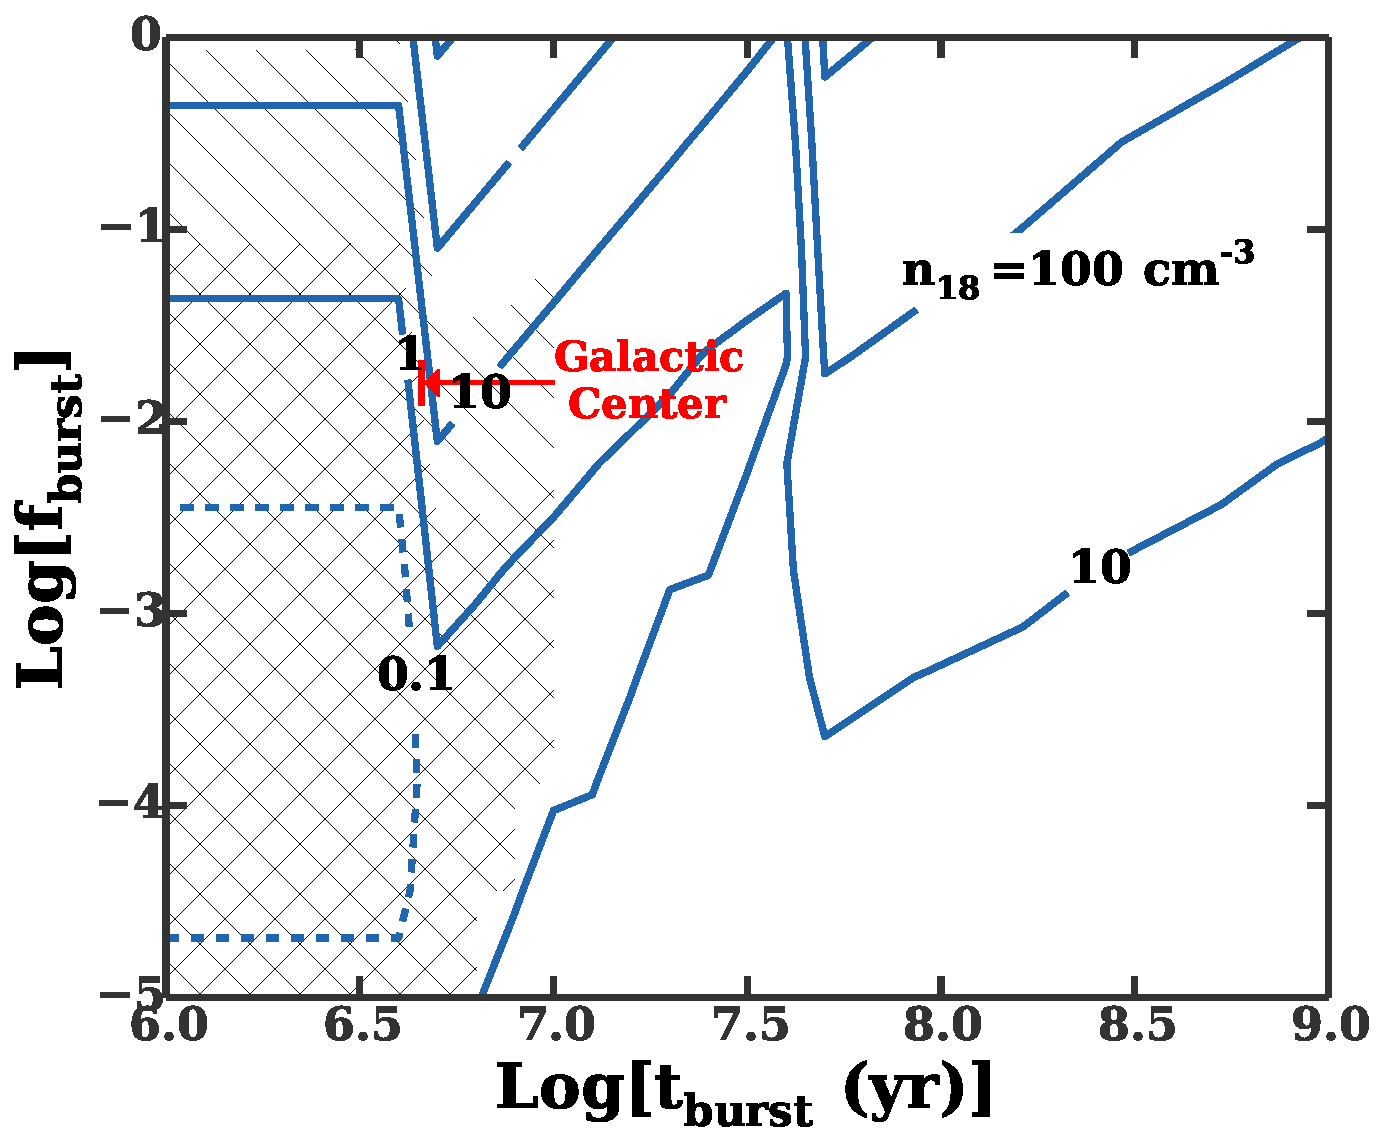
\includegraphics[width=8cm]{cnm_plot.pdf}
  \caption{\label{fig:param} Heating rates ($v_w$) and mass return
    parameters ($\eta$) for different star formation histories (gray
    lines). Solid, gray lines correspond to a star-burst of $<3$ Myr
    ago forming a fraction $f$ of the stars. The rest of the stars
    formed either a Hubble time ago (top line) or 1 Gyr ago (bottom
    line). The fraction $f$ increases and the gas density from left to
    right along these lines. The dashed, gray line corresponds to an
    alternate scenario in which there are two recent bursts in rapid
    succession in rapid succession: the older burst is $\sim 3$ Myr
    old (just at the point when stars are beginning to leave the main
    sequence). The contribution of this older burst increases towards
    the right, crossing boundary of the thermally unstable (``TI'')
    region below the thick black line.}
% Space of possible mass return parameters
%     ($\eta$) and heating rates ($v_w$) with lines of constant gas
%     density in (black lines). Red and brown lines show different star
%     formation histories... {\bf AG should include supernova heating in
%       this plot}.
\end{figure}


 


\subsection{Adopted stellar density profiles}
 Motivated by the preceding sections we adopt the following density
 profile to describe to describe the CNM of cusp galaxies

\begin{align}
n=
\begin{cases}
  n_{18} \left(\frac{r}{10^{18} {\rm cm}}\right)^{-1} {\rm cm^{-3}} & r<r_b \\
  n(r_b) \left(\frac{r}{r_b}\right)^{-\beta} {\rm cm^{-3}} & r\geq
  r_b,\\
  \label{eq:profile}
\end{cases}
\end{align}

where $0.1 \Mbh[7]^{1/2} \lsim n_{\rm 18}\lsim 2,700
\Mbh[7]^{0.38} $ cm$^{-3}$.  

The gas density density experiences a break at radius $r_b$, the break
radius in the stellar density profile, where the stellar density
transitions from an inner power law slope $\Gamma\lsim 1$ to an outer
power law slope $\beta\gsim 1$. $r_b\gsim 100$ pc for cusp galaxies,
in which case the break radius may be safely ignored as it will be
well outside the jet deceleration radius. But if there is a nuclear
star cluster present the effect $r_b$, the outer boundary of the
nuclear star cluster will correspond to a much smaller effective
$r_b\sim 1-5$ pc. 

The outer power law slope of the gas density will depend on the slope
of the $\beta$ but will typically vary between 1.5 and 2. 

We explore the parameter space of $n_{18}$, $\beta$, and $r_b$,
adopting values for these parameters summarized by
Table~\ref{tab:params} below


\begin{table}
\caption{\label{tab:params} Summary of numerical parameters used for
  the CNM profile (equation~\eqref{eq:profile}). Entries in}
\begin{minipage}{\columnwidth}
\begin{tabular}{|l|l|l|}
$n_{18}$ & $r_b [{\rm pc}]$ & $\beta$\\
\hline
  2     &  -    &  -\\
  60    &  -    &  -\\
  ...   &  1    &  1.5\\
  ...   &  ...   &  2\\
  2000  &  -    &  -\\
\end{tabular}
\end{minipage}
\end{table}


{\bf AG cores...}

We also use a core galaxy profile to see how the For core galaxies the stellar density profile is not a pure power
law. To simplify things we will consider one particular slope for the
stellar density profile  $\rho_\star\sim r^{-1-\Gamma}$ with
$\Gamma=0.1$. The gas density profile may be approximated as 

\begin{align}
\begin{cases}
n=n(r_s) k(x) & 0.4 \leq x\leq 2.0\\
n = 2.0 n(r_s) (x/0.4)^{-0.95} & x < 0.4\\
n = 0.75 n(r_s) (x/2.0)^{-0.26} & 2.0< x \leq r_s/r_b\\
n \sim x^{-1.5} & x>r_s/r_b\\
\end{cases}
\end{align}

Where, 

\begin{align}
  &x=r/r_s\\\nonumber
  &k(x)=\frac{45}{19} \frac{1}{x^{3/2}} \frac{1-x^{1.9}}{9-19
      x\frac{x^{0.9}-1}{x^{1.9}-1}}
\end{align}

We consider a high density model (near the verge of thermal
instability) and a low density model (near the lower limit of what
stellar winds can give for the CNM density). The values $n(r_s)$ and
$r_s$ are given in the table below. 

\begin{table}
\begin{tabular}{|l|l|l}
 core models & $n(r_s)$ & $r_s$\\
\hline
 High & 2,500 $\Mbh[7]^{-0.32}$ cm$^{-3}$ &  4 $\times 10^{17}  
 \Mbh[7]^{0.8}$ cm\\
 Low & 0.1 $\Mbh[7]^{-0.24}$ cm$^{-3}$ & 6$\times 10^{16} \Mbh[7]$ cm
\end{tabular}
\end{table}

  \footnotesize{
    \bibliographystyle{mn2e}
    \bibliography{master}
  }

\end{document}
